% =====================================================================
%  CAPÍTULO 1. MARCO TEÓRICO
% =====================================================================
\chapter{MARCO TEÓRICO DE LA GESTIÓN DE LA CALIDAD Y DEL CONTROL DE MATERIALES EN LOSAS ALIVIANADAS CON VIGUETAS PRETENSADAS}
\label{cap:marco}

\guia{El marco teórico amplía la descripción del problema, integra la teoría con la investigación e incluye la reseña del problema en los contextos mundial, regional y nacional. Debe limitarse a lo que interesa estudiar (Taller 2). Respete la jerarquía de fuentes del docente: (1) artículos científicos, (2) tesis, (3) libros de menos de 10 años y (4) documentos técnicos. Cite todo lo que no sea de conocimiento común.}

% ---------------------------------------------------------------------
\section{Estado del arte}
\guia{Síntesis crítica (no un resumen uno por uno) de lo que se sabe sobre: (a) la gestión de la calidad y los reprocesos en la construcción; (b) el desperdicio de materiales y su medición; (c) la aplicación de SGC o planes de calidad en obras de edificación; (d) estudios sobre losas con viguetas pretensadas en Bolivia. Cierre la sección con el vacío de conocimiento que justifica esta tesis.}

% ---------------------------------------------------------------------
\section{La calidad en la construcción}

\subsection{Conceptos de calidad, control, aseguramiento y gestión de la calidad}
\guia{Definir calidad, control de la calidad, aseguramiento de la calidad y gestión de la calidad, con las definiciones de la norma ISO~9000:2026 \parencite{iso9000_2026}. Explicar la diferencia entre el control (verificar el producto) y el aseguramiento (dar confianza en que se cumplirán los requisitos).}

\subsection{Evolución del enfoque de la calidad}
\guia{Breve evolución: inspección, control estadístico, aseguramiento, gestión de la calidad total y SGC normalizados. Aportes de Deming (ciclo PHVA), Juran (trilogía de la calidad), Crosby (cero defectos y costo de la no calidad) y Feigenbaum (control total de la calidad y costos de la calidad). Cite las obras originales que consulte directamente.}

\subsection{Principios de la gestión de la calidad}
\guia{Principios de la gestión de la calidad según la norma ISO~9000:2026 (en la edición 2015 eran siete: enfoque al cliente, liderazgo, compromiso de las personas, enfoque a procesos, mejora, toma de decisiones basada en la evidencia y gestión de las relaciones; verificar los cambios en la edición vigente). Relacionar cada principio con la ejecución de una losa.}

% ---------------------------------------------------------------------
\section{Sistema de Gestión de la Calidad según la norma ISO~9001:2026}

\subsection{Estructura de la norma y ciclo PHVA}
\guia{Cláusulas 4 a 10 de la norma ISO~9001:2026 \parencite{iso9001_2026}, que conserva la estructura de alto nivel de la edición 2015: contexto, liderazgo, planificación, apoyo, operación, evaluación del desempeño y mejora. Presentar un esquema del ciclo PHVA aplicado al proceso constructivo de la losa.}

\subsection{Pensamiento basado en riesgos}
\guia{Riesgos y oportunidades (cláusula 6.1). Ejemplos en la losa: rotura de viguetas, falta de apuntalamiento, segregación del hormigón y curado insuficiente.}

\subsection{Planes de la calidad para proyectos}
\guia{Contenido de un plan de la calidad según la norma ISO~10005:2018 \parencite{iso10005_2018}: alcance, entradas, objetivos, responsabilidades, control de documentos y registros, recursos, compras, control de la producción, seguimiento y medición, no conformidades y auditoría. Mencionar la ISO~10006 (gestión de la calidad en proyectos) y el enfoque del PMI (planificar, gestionar y controlar la calidad).}

% ---------------------------------------------------------------------
\section{Costos de la calidad}

\subsection{Modelo de prevención, evaluación y fallas}
\guia{Modelo PAF: costos de prevención (planificación, capacitación), de evaluación (inspecciones y ensayos), de fallas internas (desperdicio, retrabajo, reparación) y de fallas externas (correcciones posteriores a la entrega, reclamos, sobremediciones corregidas, ampliaciones). Mostrar la relación entre la inversión en prevención y evaluación y la reducción de las fallas.}

\subsection{Costo de no calidad y reprocesos en la construcción}
\guia{Definición de reproceso (\emph{rework}) y sus causas. Cifras de referencia: reprocesos de hasta 12,4~\% del costo del proyecto, con un promedio de 6,59~\% \parencite{alvarez2014}; impacto de los reprocesos en el desempeño de costos \parencite{hwang2009}. Agregar estudios latinoamericanos y bolivianos.}

% ---------------------------------------------------------------------
\section{Pérdidas y desperdicio de materiales en la construcción}

\subsection{Clasificación y causas de las pérdidas}
\guia{Tipos de pérdidas: material que se convierte en residuo, material incorporado en exceso (sobreespesores, sobreconsumo) y pérdidas por robo o daño. Causas según su origen: diseño, suministro, almacenamiento, manipulación, ejecución y gestión.}

\subsection{Índices de desperdicio y su medición}
\guia{Definir el índice de desperdicio de materiales como la diferencia entre la cantidad real y la teórica, dividida entre la teórica. Explicar cómo se obtienen la cantidad teórica (planos y cómputos) y la real (kardex, entregas, conteo, volúmenes vaciados). Presentar valores de referencia de la bibliografía para hormigón, acero, bloques y otros insumos.}

\subsection{Enfoque Lean Construction para reducir pérdidas}
\guia{Principios de la construcción sin pérdidas: flujo, reducción de la variabilidad, planificación colaborativa y mejora continua. Relación con el SGC.}

% ---------------------------------------------------------------------
\section{Losas alivianadas con viguetas pretensadas y complemento de plastoformo}

\subsection{Descripción del sistema y de sus componentes}

La losa alivianada del Edificio de Posgrado es una losa nervada unidireccional compuesta por:
\begin{itemize}
  \item viguetas pretensadas de fabricación industrial;
  \item complementos de poliestireno expandido (plastoformo);
  \item nervios transversales rigidizadores;
  \item una carpeta de compresión de hormigón vaciado en obra.
\end{itemize}

Las especificaciones técnicas del proyecto \parencite{uatf_et} establecen los siguientes requisitos:
\begin{itemize}
  \item \textbf{Viguetas:} hormigón de 350 a 400~kg/cm\textsuperscript{2}, acero con tensión de rotura de 18.000~kg/cm\textsuperscript{2} y certificación IBNORCA e ISO.
  \item \textbf{Complementos:} bloques de plastoformo de 100~$\times$~50~$\times$~20~cm.
  \item \textbf{Carpeta de compresión:} hormigón de resistencia característica de 250~kg/cm\textsuperscript{2}, con un contenido mínimo de cemento de 400~kg/\mtres{}.
\end{itemize}

El certificado de calidad del fabricante de las viguetas indica una separación entre ejes de 50~cm, un espesor de losa de 20~+~5~=~25~cm, una sobrecarga admisible de 400~kg/\mdos{} y una luz máxima de 7,50~m en condición simplemente apoyada \parencite{pretensa2025}. La Figura~\ref{fig:seccion} muestra la sección típica de la losa. La Figura~\ref{fig:corte} muestra el corte transversal con la armadura de distribución de $\phi$6~c/20~cm en ambas direcciones.

\begin{figure}[H]
\centering
\caption{Sección típica de la losa alivianada con viguetas pretensadas}
\label{fig:seccion}
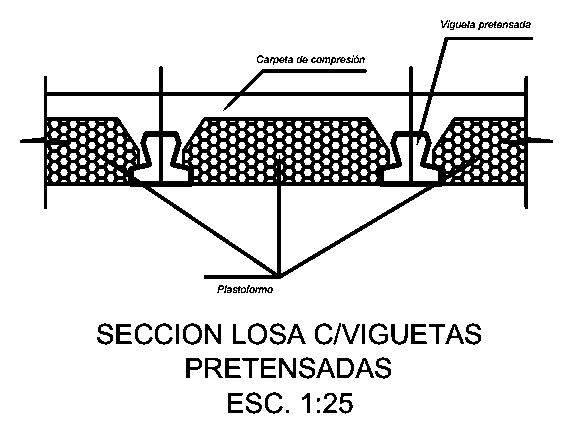
\includegraphics[width=0.60\linewidth]{plano02_seccion_losa_viguetas}
\nota{Tomado del Plano~02 del proyecto «Construcción Edificio de Posgrado» de la UATF.}
\end{figure}

\begin{figure}[H]
\centering
\caption{Corte transversal de la losa con la carpeta de compresión y la armadura de distribución}
\label{fig:corte}
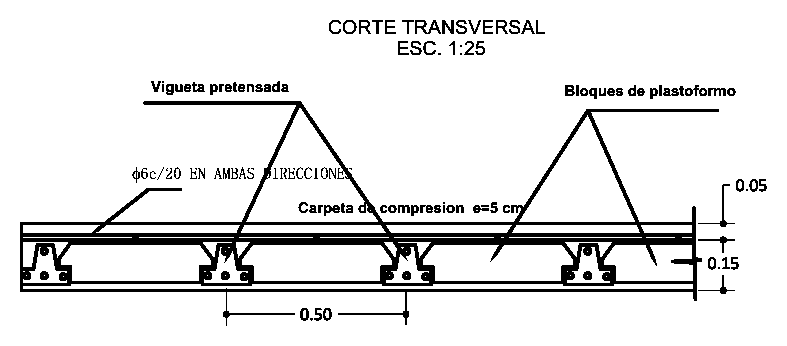
\includegraphics[width=0.85\linewidth]{plano02_corte_transversal}
\nota{Tomado del Plano~02 del proyecto. El corte acota 0,15~m de altura de complemento y 0,05~m de carpeta, mientras que las especificaciones técnicas y el certificado del fabricante indican 20~+~5~cm. Esta discrepancia se analiza en la sección~\ref{sec:analisis-documental}.}
\end{figure}

\subsection{Proceso constructivo}
\guia{Describir la secuencia de ejecución:
\begin{enumerate}
  \item replanteo;
  \item apuntalamiento y encofrado de vigas;
  \item colocación de viguetas y complementos;
  \item nervios transversales;
  \item armadura de distribución y de momentos negativos;
  \item instalaciones embebidas (ductos y cajas eléctricas y sanitarias);
  \item limpieza y humedecido;
  \item hormigonado y vibrado;
  \item curado;
  \item desapuntalamiento.
\end{enumerate}
Para cada actividad, indicar los puntos críticos de calidad. Usar el manual del fabricante y las especificaciones técnicas.}

\subsection{Consumos teóricos de materiales por metro cuadrado}
\guia{Calcular con los planos (Plano~03: cantidad de viguetas por paño) y la sección típica:
\begin{itemize}
  \item metros de vigueta por \mdos{};
  \item piezas de complemento por \mdos{};
  \item volumen de hormigón por \mdos{} (carpeta + nervios);
  \item kilogramos de acero por \mdos{} (malla de $\phi$6~c/20 + negativos + nervios).
\end{itemize}
Estos valores son la «cantidad teórica» del índice de desperdicio. Como referencia, el cómputo de acero de la losa de la obra da 4.171,18~kg para 1.109,84~\mdos{}, es decir, $\approx$~3,76~kg/\mdos{} \parencite{uatf_pao3}.}

\subsection{Defectos y fallas frecuentes}
\guia{Fisuras, flechas excesivas, segregación y nidos de grava, recubrimiento insuficiente, viguetas dañadas, desplazamiento de complementos durante el vaciado y falta de continuidad de la armadura negativa. Indicar sus causas y cómo prevenirlos.}

% ---------------------------------------------------------------------
\section{Marco normativo}

\subsection{Normas de gestión de la calidad}
\guia{ISO~9000:2026 y NB/ISO~9000:2026 (fundamentos y vocabulario); ISO~9001:2026 y NB/ISO~9001:2026 (requisitos; sustituyen a la edición 2015, cuyos certificados tienen un periodo de transición); ISO~10005:2018 y NB/ISO~10005:2021 (planes de la calidad); ISO~10006:2017 y NB/ISO~10006:2021 (calidad en proyectos); ISO~10014:2021 y NB/ISO~10014:2022 (beneficios financieros y económicos de la calidad).}

\subsection{Normas de hormigón estructural}
\guia{La CBH-87, citada en las especificaciones del proyecto, sigue siendo la norma de hormigón declarada obligatoria por decreto (D.~S.~22976 de 1991). La norma técnica actual es la NB~1225001-1:2017 (IBNORCA), basada en el código ACI~318 y ratificada por el MOPSV en 2020, aún no elevada a decreto supremo \pendiente{confirmar}. Declarar qué criterio de aceptación del hormigón se adopta y por qué. Código ACI~318-25 \parencite{aci318_2025}: capítulo~26 (documentos de construcción e inspección), muestreo (26.12.2), criterios de aceptación (26.12.3) y curado (26.5.3).}

\subsection{Norma de viguetas pretensadas}
\guia{NB~997:2016, «Elementos prefabricados de hormigón -- Viguetas prefabricadas de hormigón pretensado -- Requisitos y métodos de ensayo» (IBNORCA), citada en el certificado del fabricante \parencite{pretensa2025}. Usarla para los criterios de recepción de viguetas.}

\subsection{Normas de ensayo}
\guia{ASTM C172 (muestreo del hormigón fresco), C31 (elaboración y curado de probetas en obra), C143 (asentamiento), C39 (resistencia a compresión de cilindros), C94 (hormigón premezclado, si corresponde) y A615 (barras corrugadas), junto con sus equivalentes bolivianas: NB~634 (toma de muestras), NB~586 (probetas), NB~589 (cono de Abrams), NB~639 (compresión) y NB~736 y NB~739 (barras de acero) \pendiente{verificar equivalencias y años}. Indicar qué controla cada una en la losa.}

\subsection{Normativa de contratación pública}
\guia{Ley~1178 (SAFCO) y D.~S.~0181 (NB-SABS): funciones de la Supervisión y la Fiscalización, Libro de Órdenes, planillas de avance, órdenes de cambio, contratos modificatorios y sus límites porcentuales, y resolución de contrato. Según el artículo 89 del D.~S.~0181, los contratos modificatorios no pueden superar el 10~\% del monto del contrato y las órdenes de cambio el 5~\% (15~\% en conjunto en licitación pública). Incluir los decretos de ajuste excepcional de precios (D.~S.~5321 de 2025 y D.~S.~5597 de 2026). Relacionar con los hechos del caso (contrato modificatorio del 7,22~\% y resolución).}

% ---------------------------------------------------------------------
\section{Control de costos en obras públicas}
\guia{Análisis de precios unitarios (materiales, mano de obra, equipo, gastos generales, utilidad e impuestos), cómputos métricos, planillas de avance y certificados de pago. Explicar cómo el desperdicio y los reprocesos afectan al costo real frente al costo contractual. Mencionar el reajuste de precios por alza de insumos (2025--2026).}

% ---------------------------------------------------------------------
\section{Herramientas de la calidad}
\guia{Hoja de verificación, diagrama de Pareto, diagrama de Ishikawa, histograma, cartas de control, plan de puntos de inspección (PPI) y técnica 5W2H. Para cada una: para qué sirve y cómo se aplicará en esta tesis.}

% ---------------------------------------------------------------------
\section{Definición de términos básicos}
\guia{Glosario breve: calidad, conformidad, no conformidad, acción correctiva, desperdicio, reproceso, punto de inspección, liberación de actividad, trazabilidad, lote, f'c, asentamiento, carpeta de compresión, vigueta pretensada, complemento y apuntalamiento.}
